\subsection{担保金额汇总问题}
具体问题描述可见 \ref{pro3} 担保金额汇总问题一节.

备注: 此问题我们花了大量时间与精力,但是没有解决,我们进行了两次修改,但都以失
败告终,但是仍有很大收获。

此问题涉及的数据文件有:
\begin{itemize}
  \item Person.csv(点)
  \item Loan.csv(点)
  \item PersonApplyLoan.csv(边)
  \item PersonGuarantee.csv(边)
\end{itemize}

\subsubsection{思路历程}
根据题目需分两步走,首先我们需要知道 person 所 guarantee 的 person 的 loan
的 amount 信息,所以,我们打算先将 Person.csv 和 Loan.csv 与 PersonApplyLoan 连接起来,
得出一张包含 personid 和此 person 所 apply 的 loan 的 amount 总和两个字段的新表,接着第二步,
根据这张新表与 personguaranteeperson 表,再去分析 person 下游的人找到满足要求的
person 信息。

\subsubsection{代码分析与实现}
由于在此项目中,分为点文件和边文件,可以抽象理解为根据输入的点和边,点具有 id 和
value 两个属性,边具有起始点 id 和终点 id 和 value 三个属性,调用接口后为抽象成一幅图,
可以对图(所有点)进行迭代,遍历等操作。于是,我们先将person和loan都当作点,点
的 id 即为 person 或 loan 对应的 id,而对于 value 值,我们将 loan 的 value 设为其 amount,将
person的value设为0,对于边,将value设置为空字符串,通过输入流 pwindowsource 分别
进行输入。接着我们用 buildwindowstreamgraph 进行构图,在构图中我们用 union 操作将
loan 和 person 点合并在一起,代码如下:
\begin{figure}[H]
  \begin{center}
    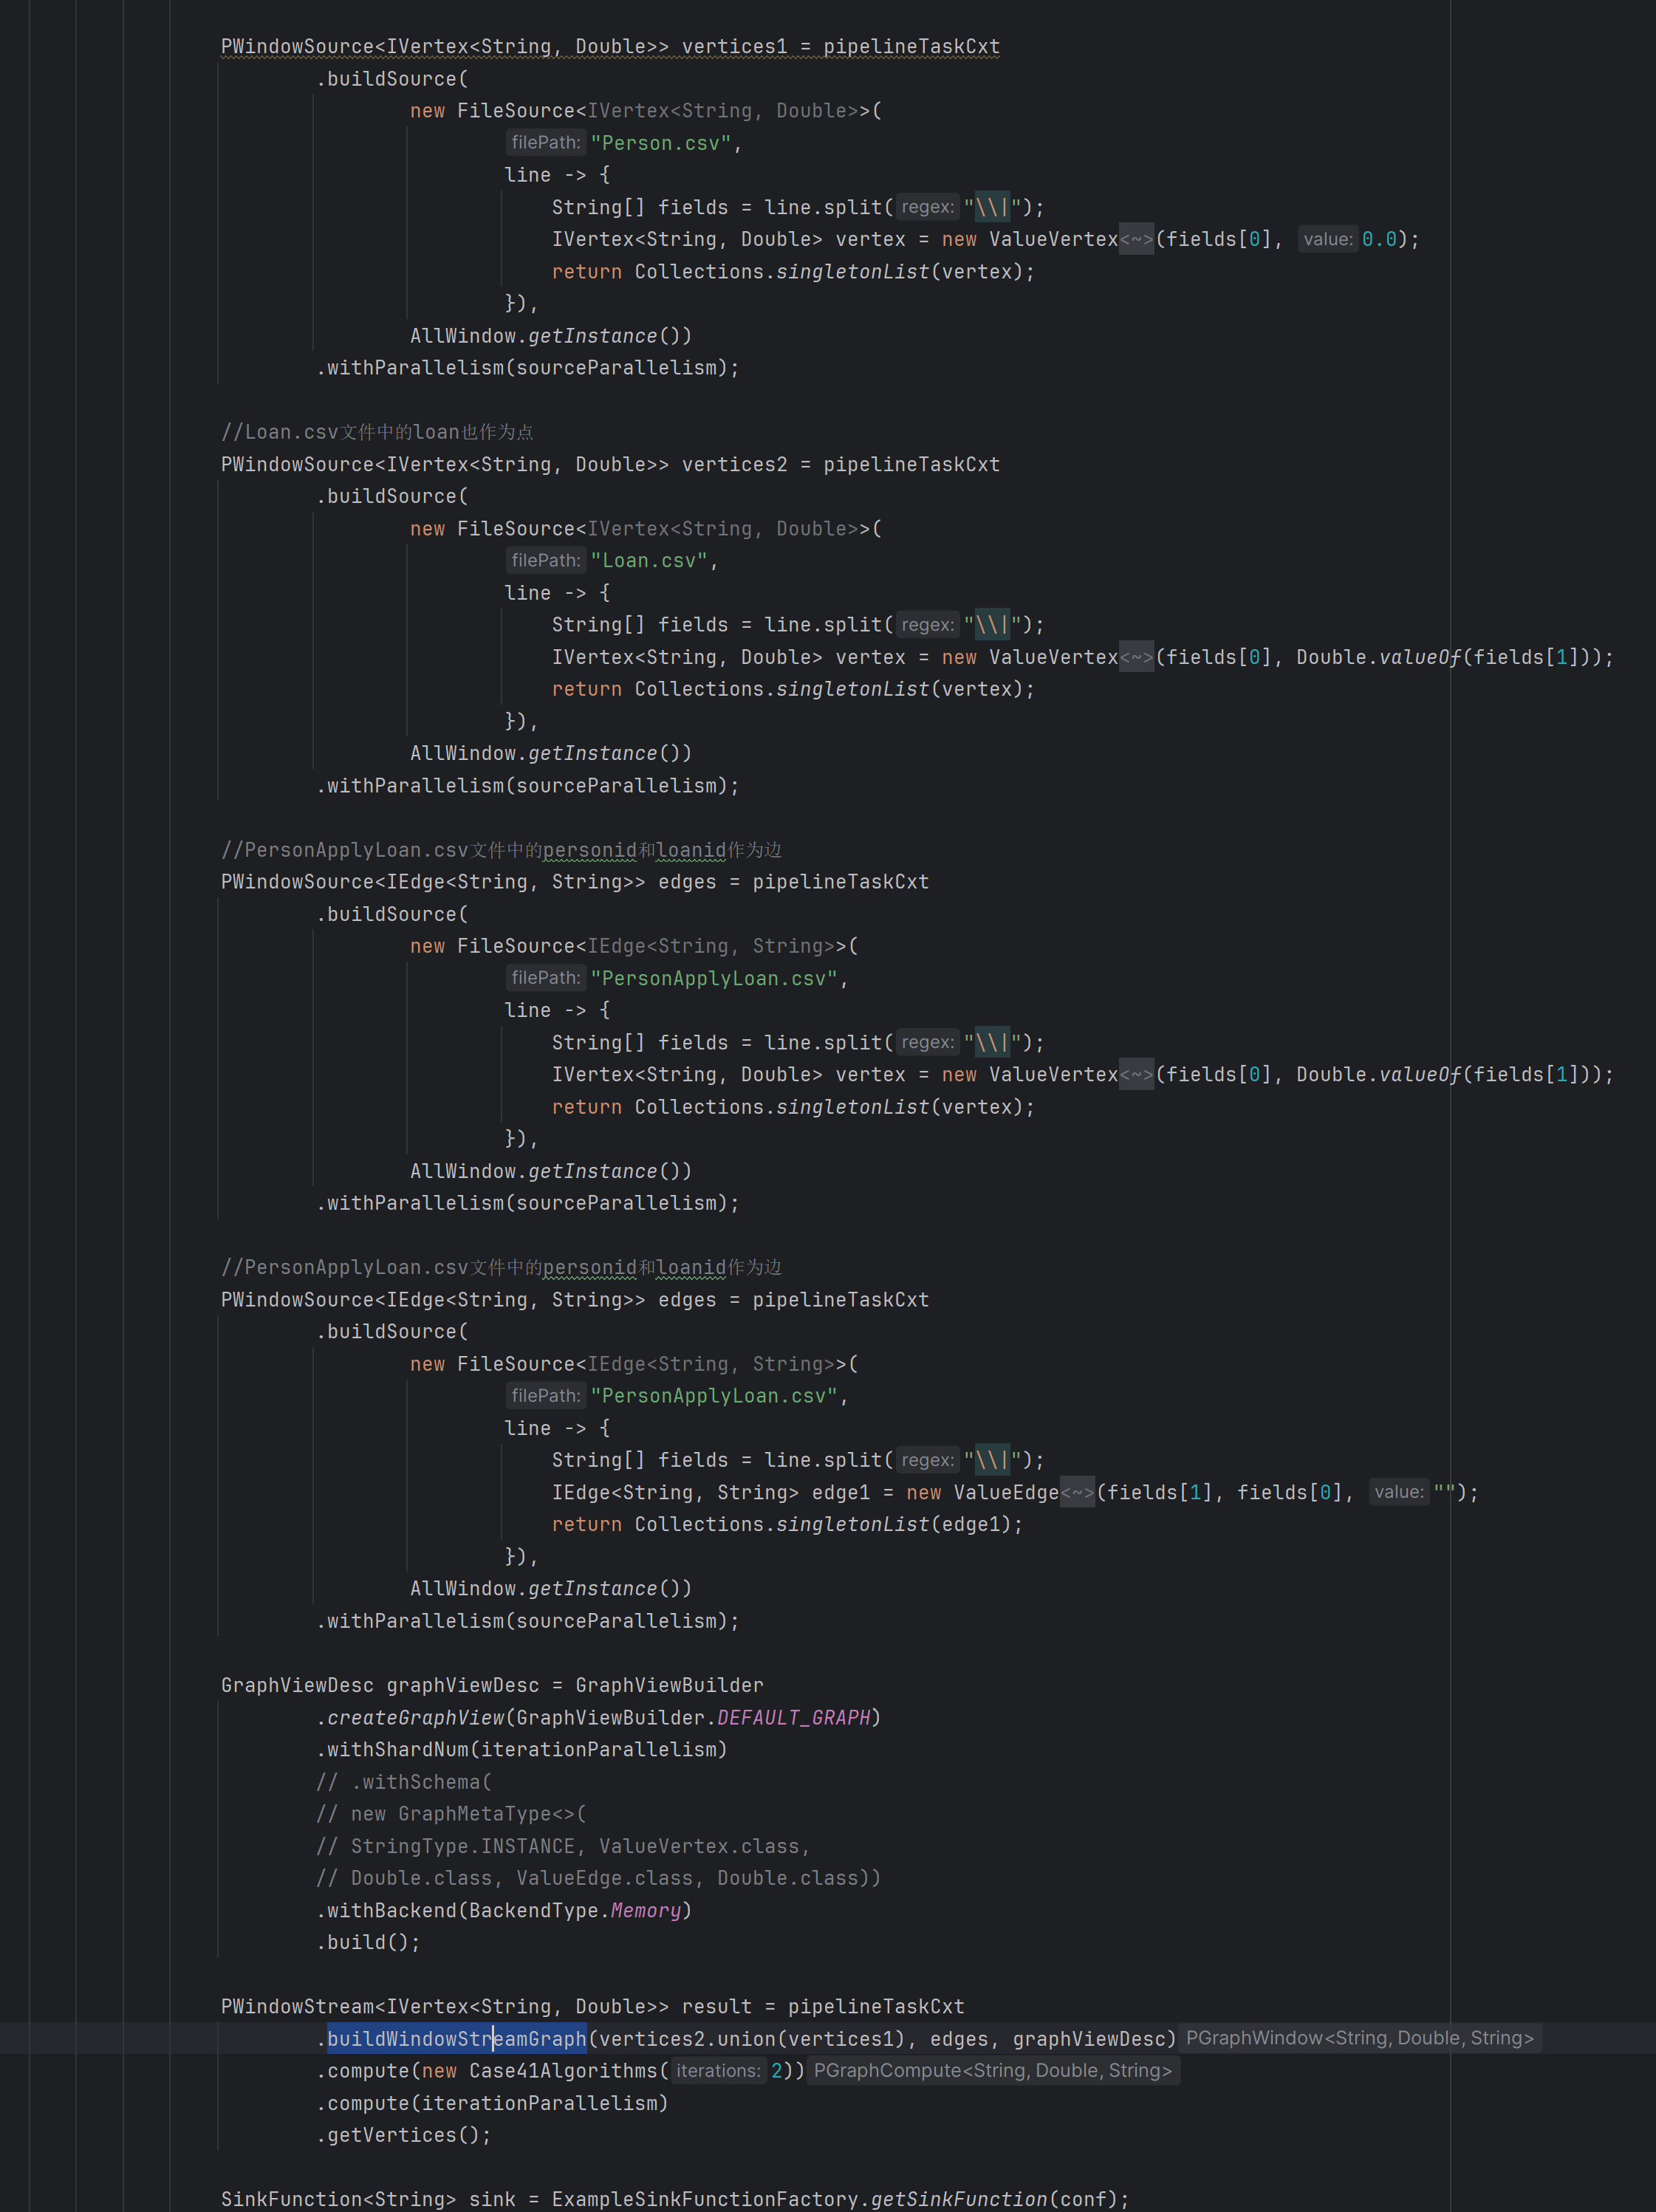
\includegraphics[width=0.85\textwidth,scale=0.7]{./figures/pro3/1.png}
  \end{center}
\end{figure}

接着我们需要得出一个新文件让每个person带上amount,于是,算法思路是进行对所有点
进行两轮迭代,第一轮所有点迭代中,让所有拥有出边的loan点(即此loan有至少一个人
apply),向所有出边的目标点(即person点)发送自己的amount值。最后将自己的value
值设置为 $ -1 $
以方便后续的过滤。(区分person点和loan点的方式是value值是否大于0)

在第二轮迭代中,由于每个点都有一个接收器,我们让所有接收器不为空的点(即person点)
计算接收器的总和 sum 并将 value 值更新为 sum,
到这一步,所有 person 的 value 值 $ >=0 $,所有 loan 的 value 值都为 $ -1 $,
核心代码如下:
\begin{figure}[H]
  \begin{center}
    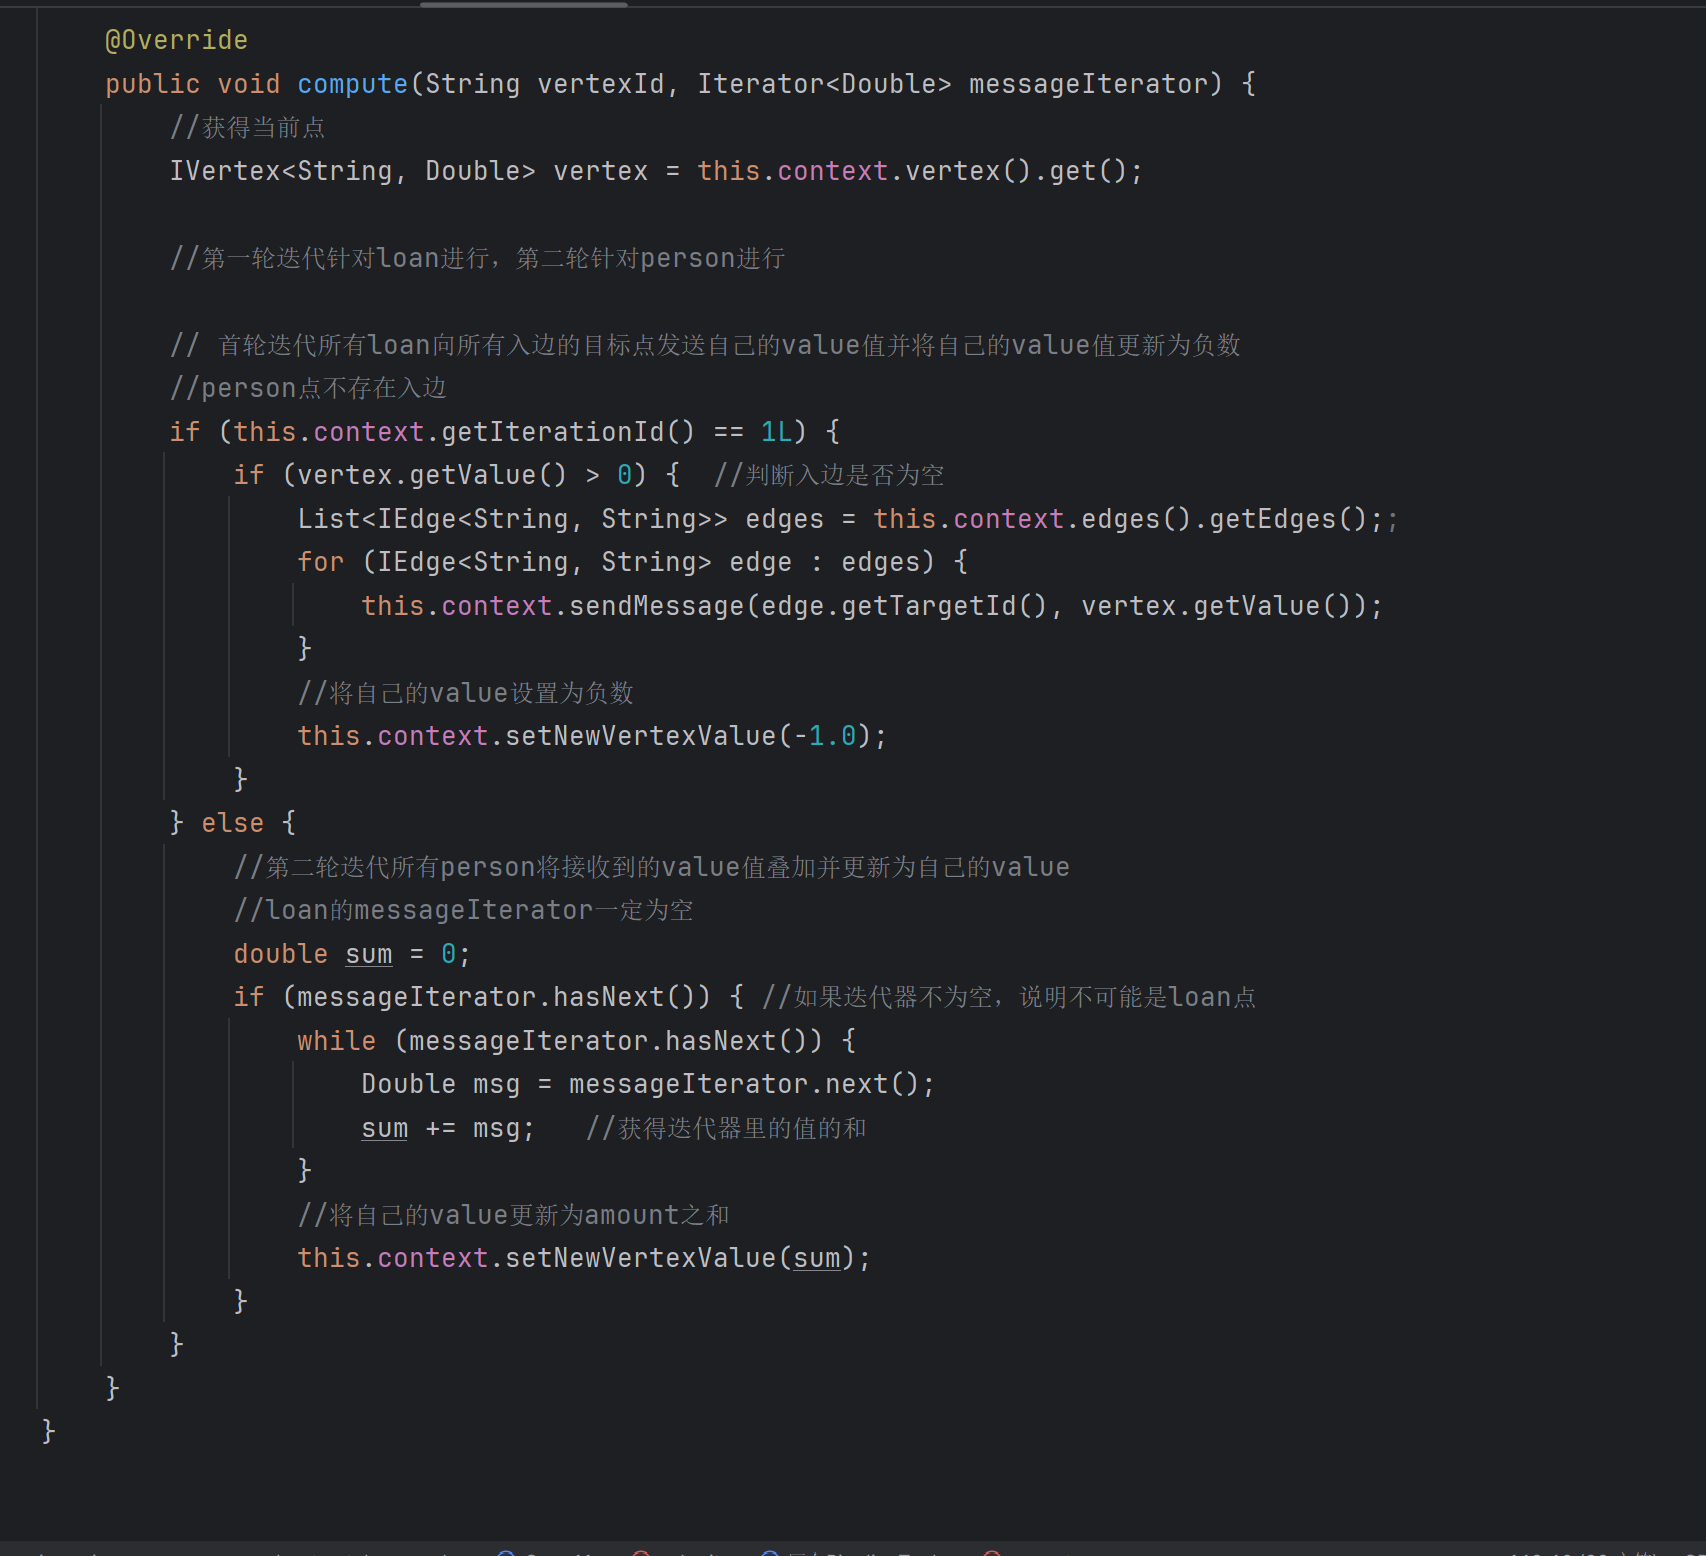
\includegraphics[width=0.85\textwidth,scale=0.7]{./figures/pro3/2.png}
  \end{center}
\end{figure}

最后,将所有点进行过滤涤除value 小于 $ 0 $ 的点(即loan点)得到中间文件。
\begin{figure}[H]
  \begin{center}
    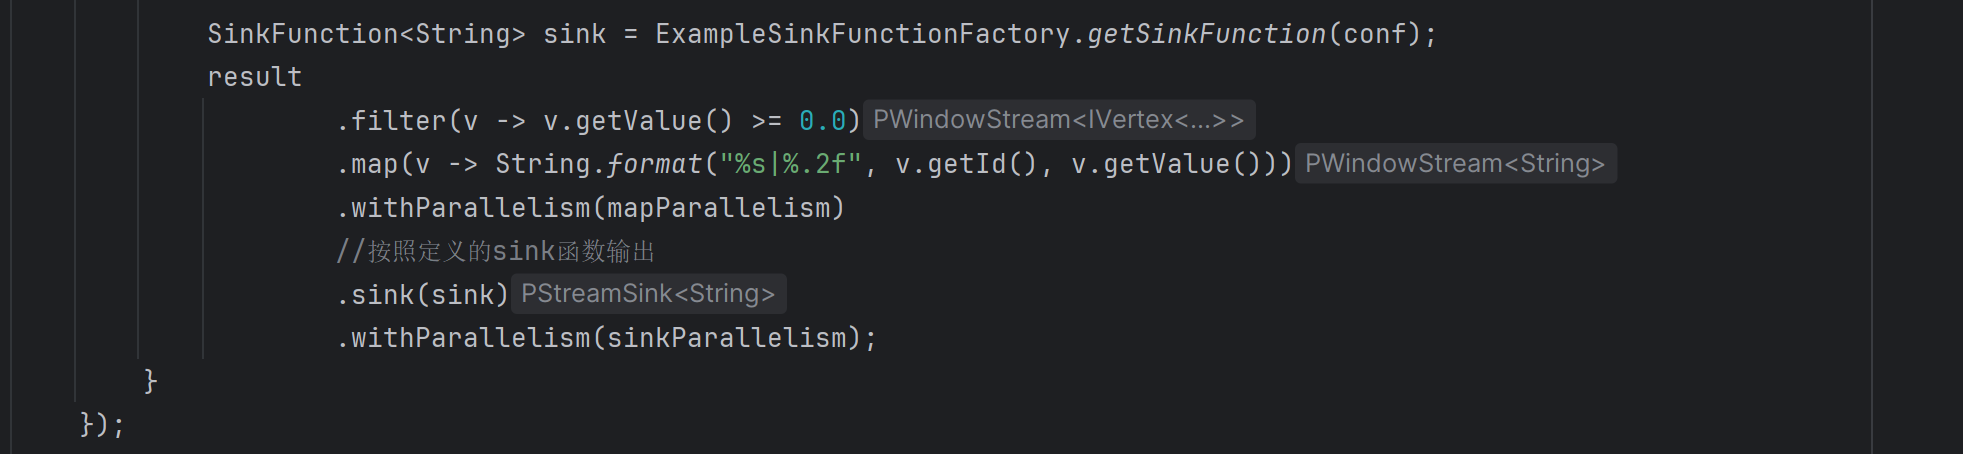
\includegraphics[width=0.85\textwidth,scale=0.7]{./figures/pro3/3.png}
  \end{center}
\end{figure}

接着进入第二步操作,首先因为我们要将中间文件与personguaranteeperson文件联合起来
构建成图,点的id为person的id,点的value为person的value,边的value为空字符串:
\begin{figure}[H]
  \begin{center}
    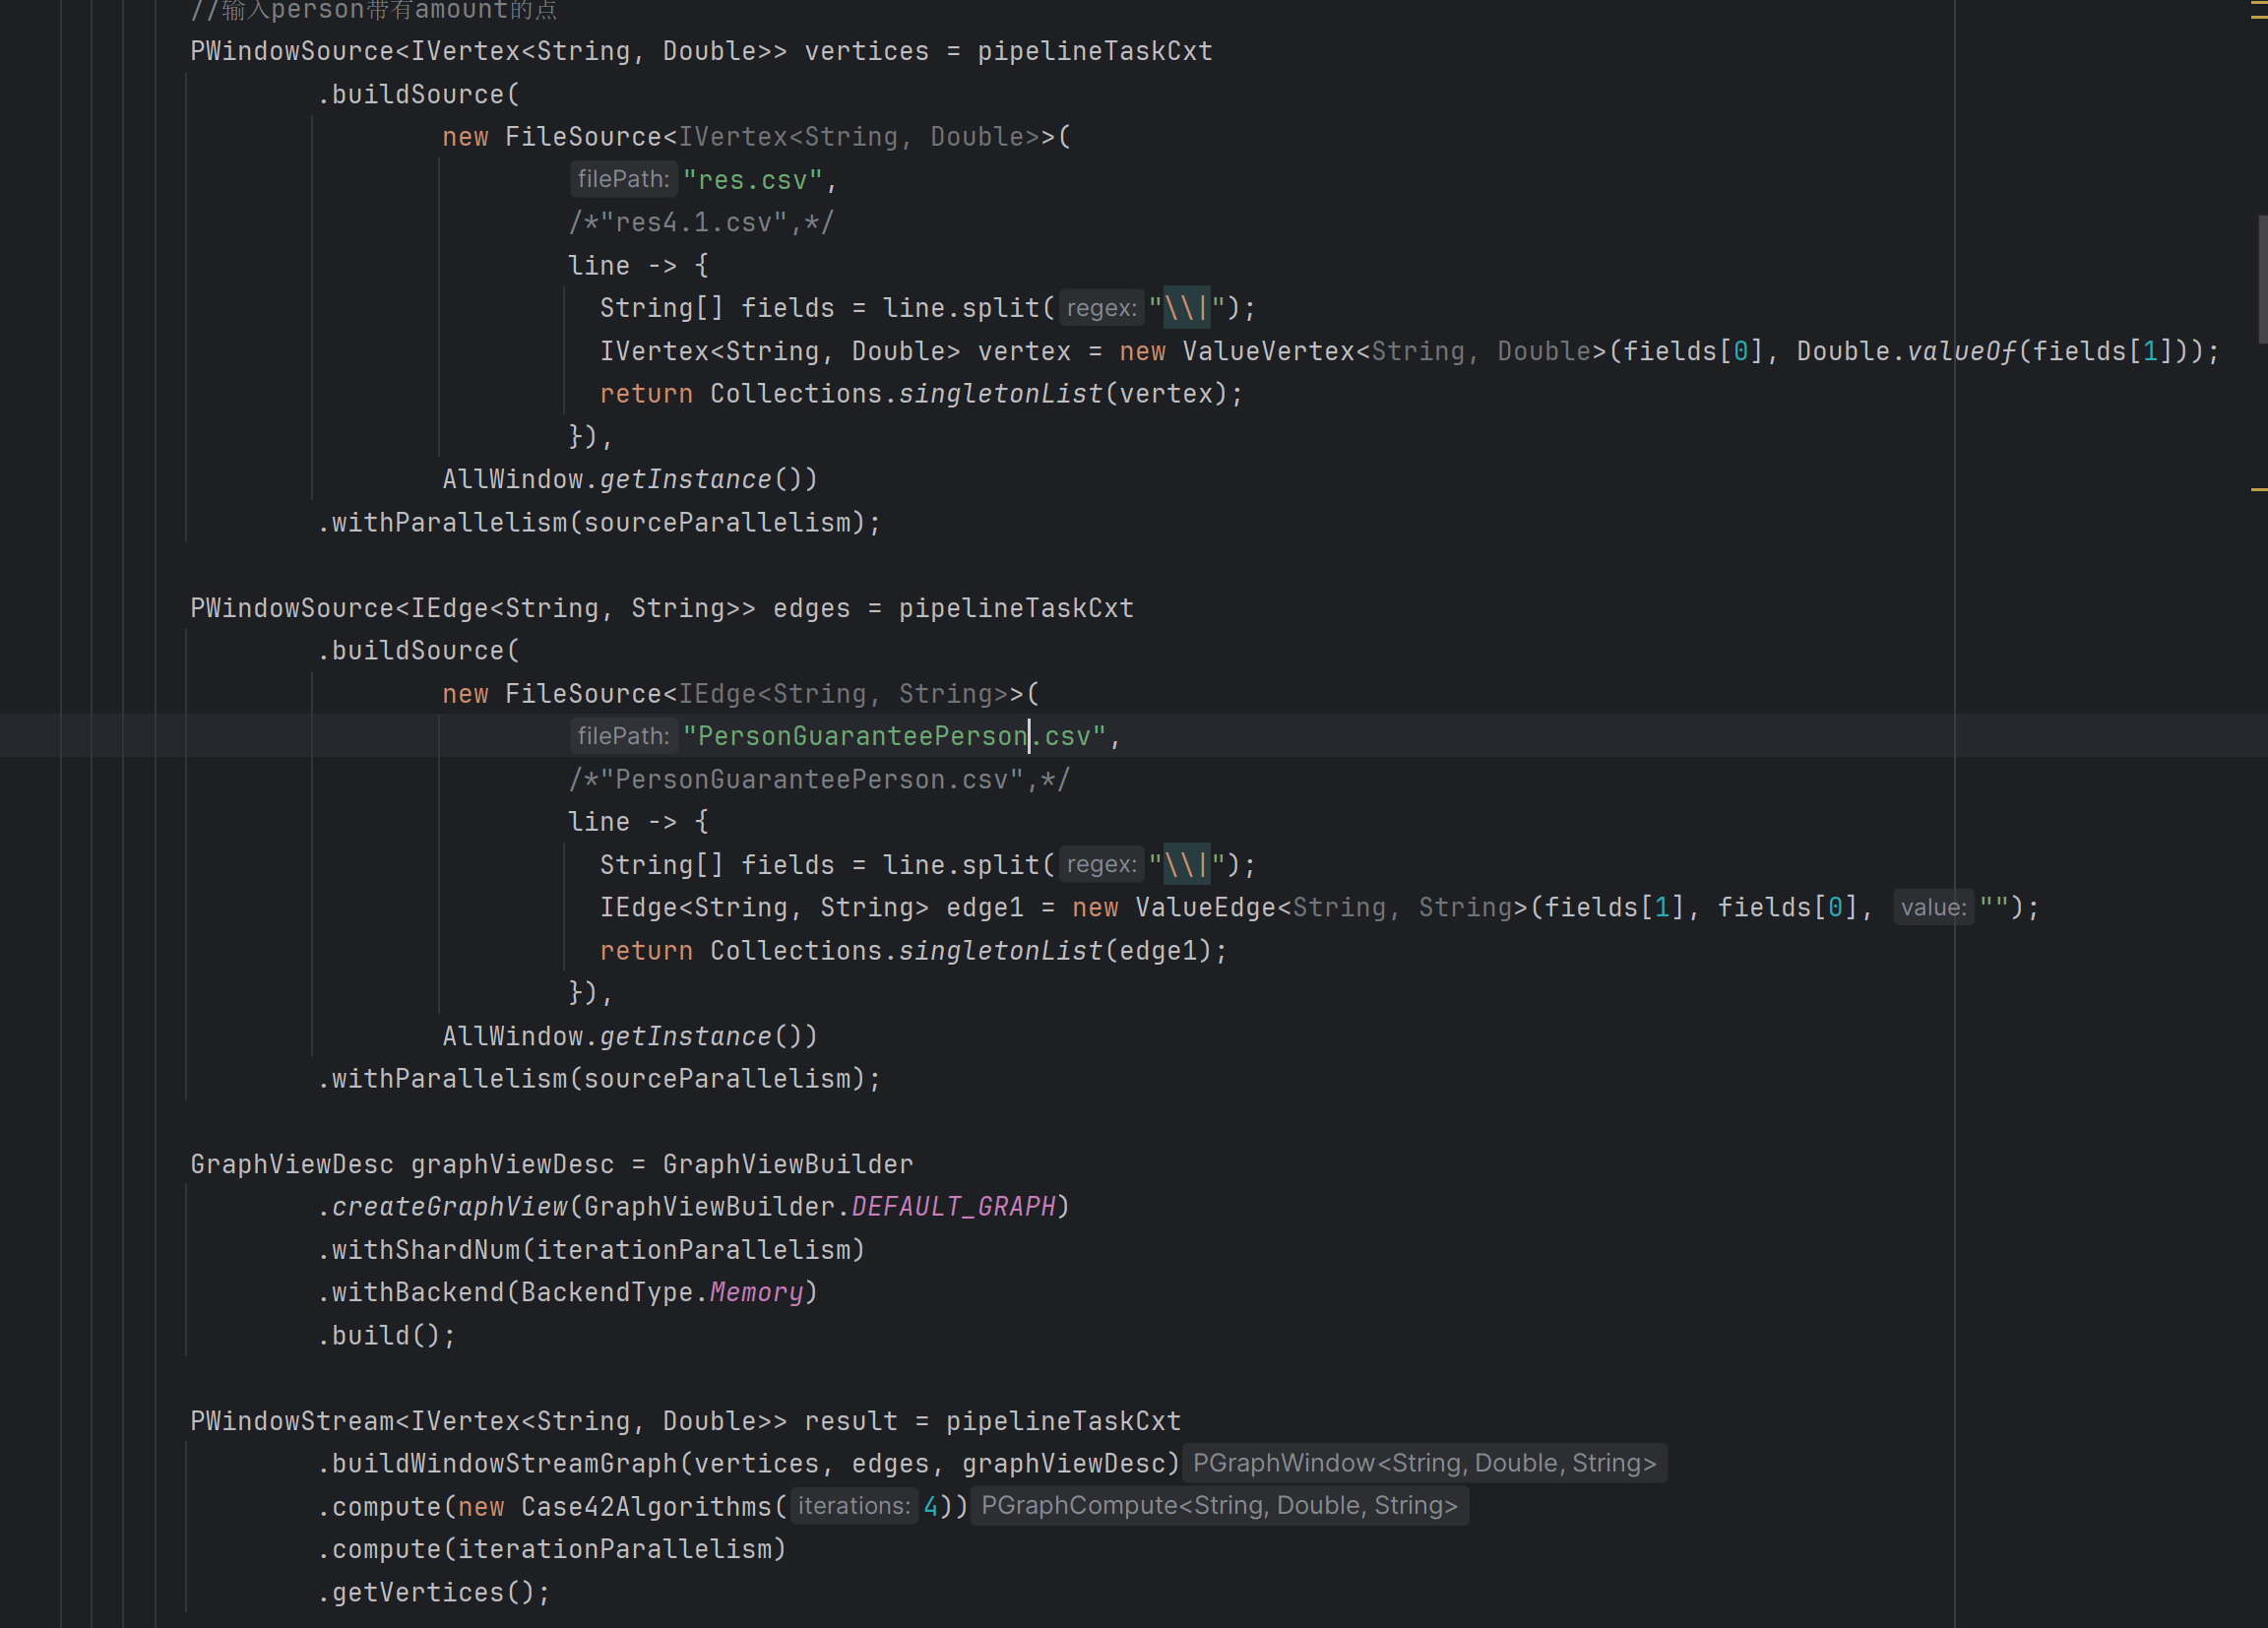
\includegraphics[width=0.85\textwidth,scale=0.7]{./figures/pro3/4.png}
  \end{center}
\end{figure}

接着我们进行四轮迭代,核心思想是在第n轮迭代中,所有点的value值都用来存储其下n-1
级所有点的amount总和。第一轮迭代中,所有点向它的所有出边目标点发送自己的value
值即amount值,在第二轮迭代中让点计算接收器的值sum并将value值更新为sum,同时继
续向此点的所有出边点发送自己的value值,在第二轮迭代完成后每一个点的value值都是
其下一级所有点的amount总和。在第三轮迭代中所有点计算接收器中的总和sum,接着继
续向所有出边点发送sum,同时更新自己的value值为sum+value。第三轮迭代结束后所有
点的value值即为其下两级所有点的amount总和。在第四轮迭代中所有点重复第三轮迭代
的更新操作并得到最终结果。
需要注意的是,接收器每一轮都会进行更新,只存储新的接收值,同时,接收器没接收信
息的点将不会进入下一轮迭代,这就是为什么在下面代码中我们让所有点都向自己的接收
器发送 $ 0.0 $(不影响结果)。核心代码如下:
\begin{figure}[H]
  \begin{center}
    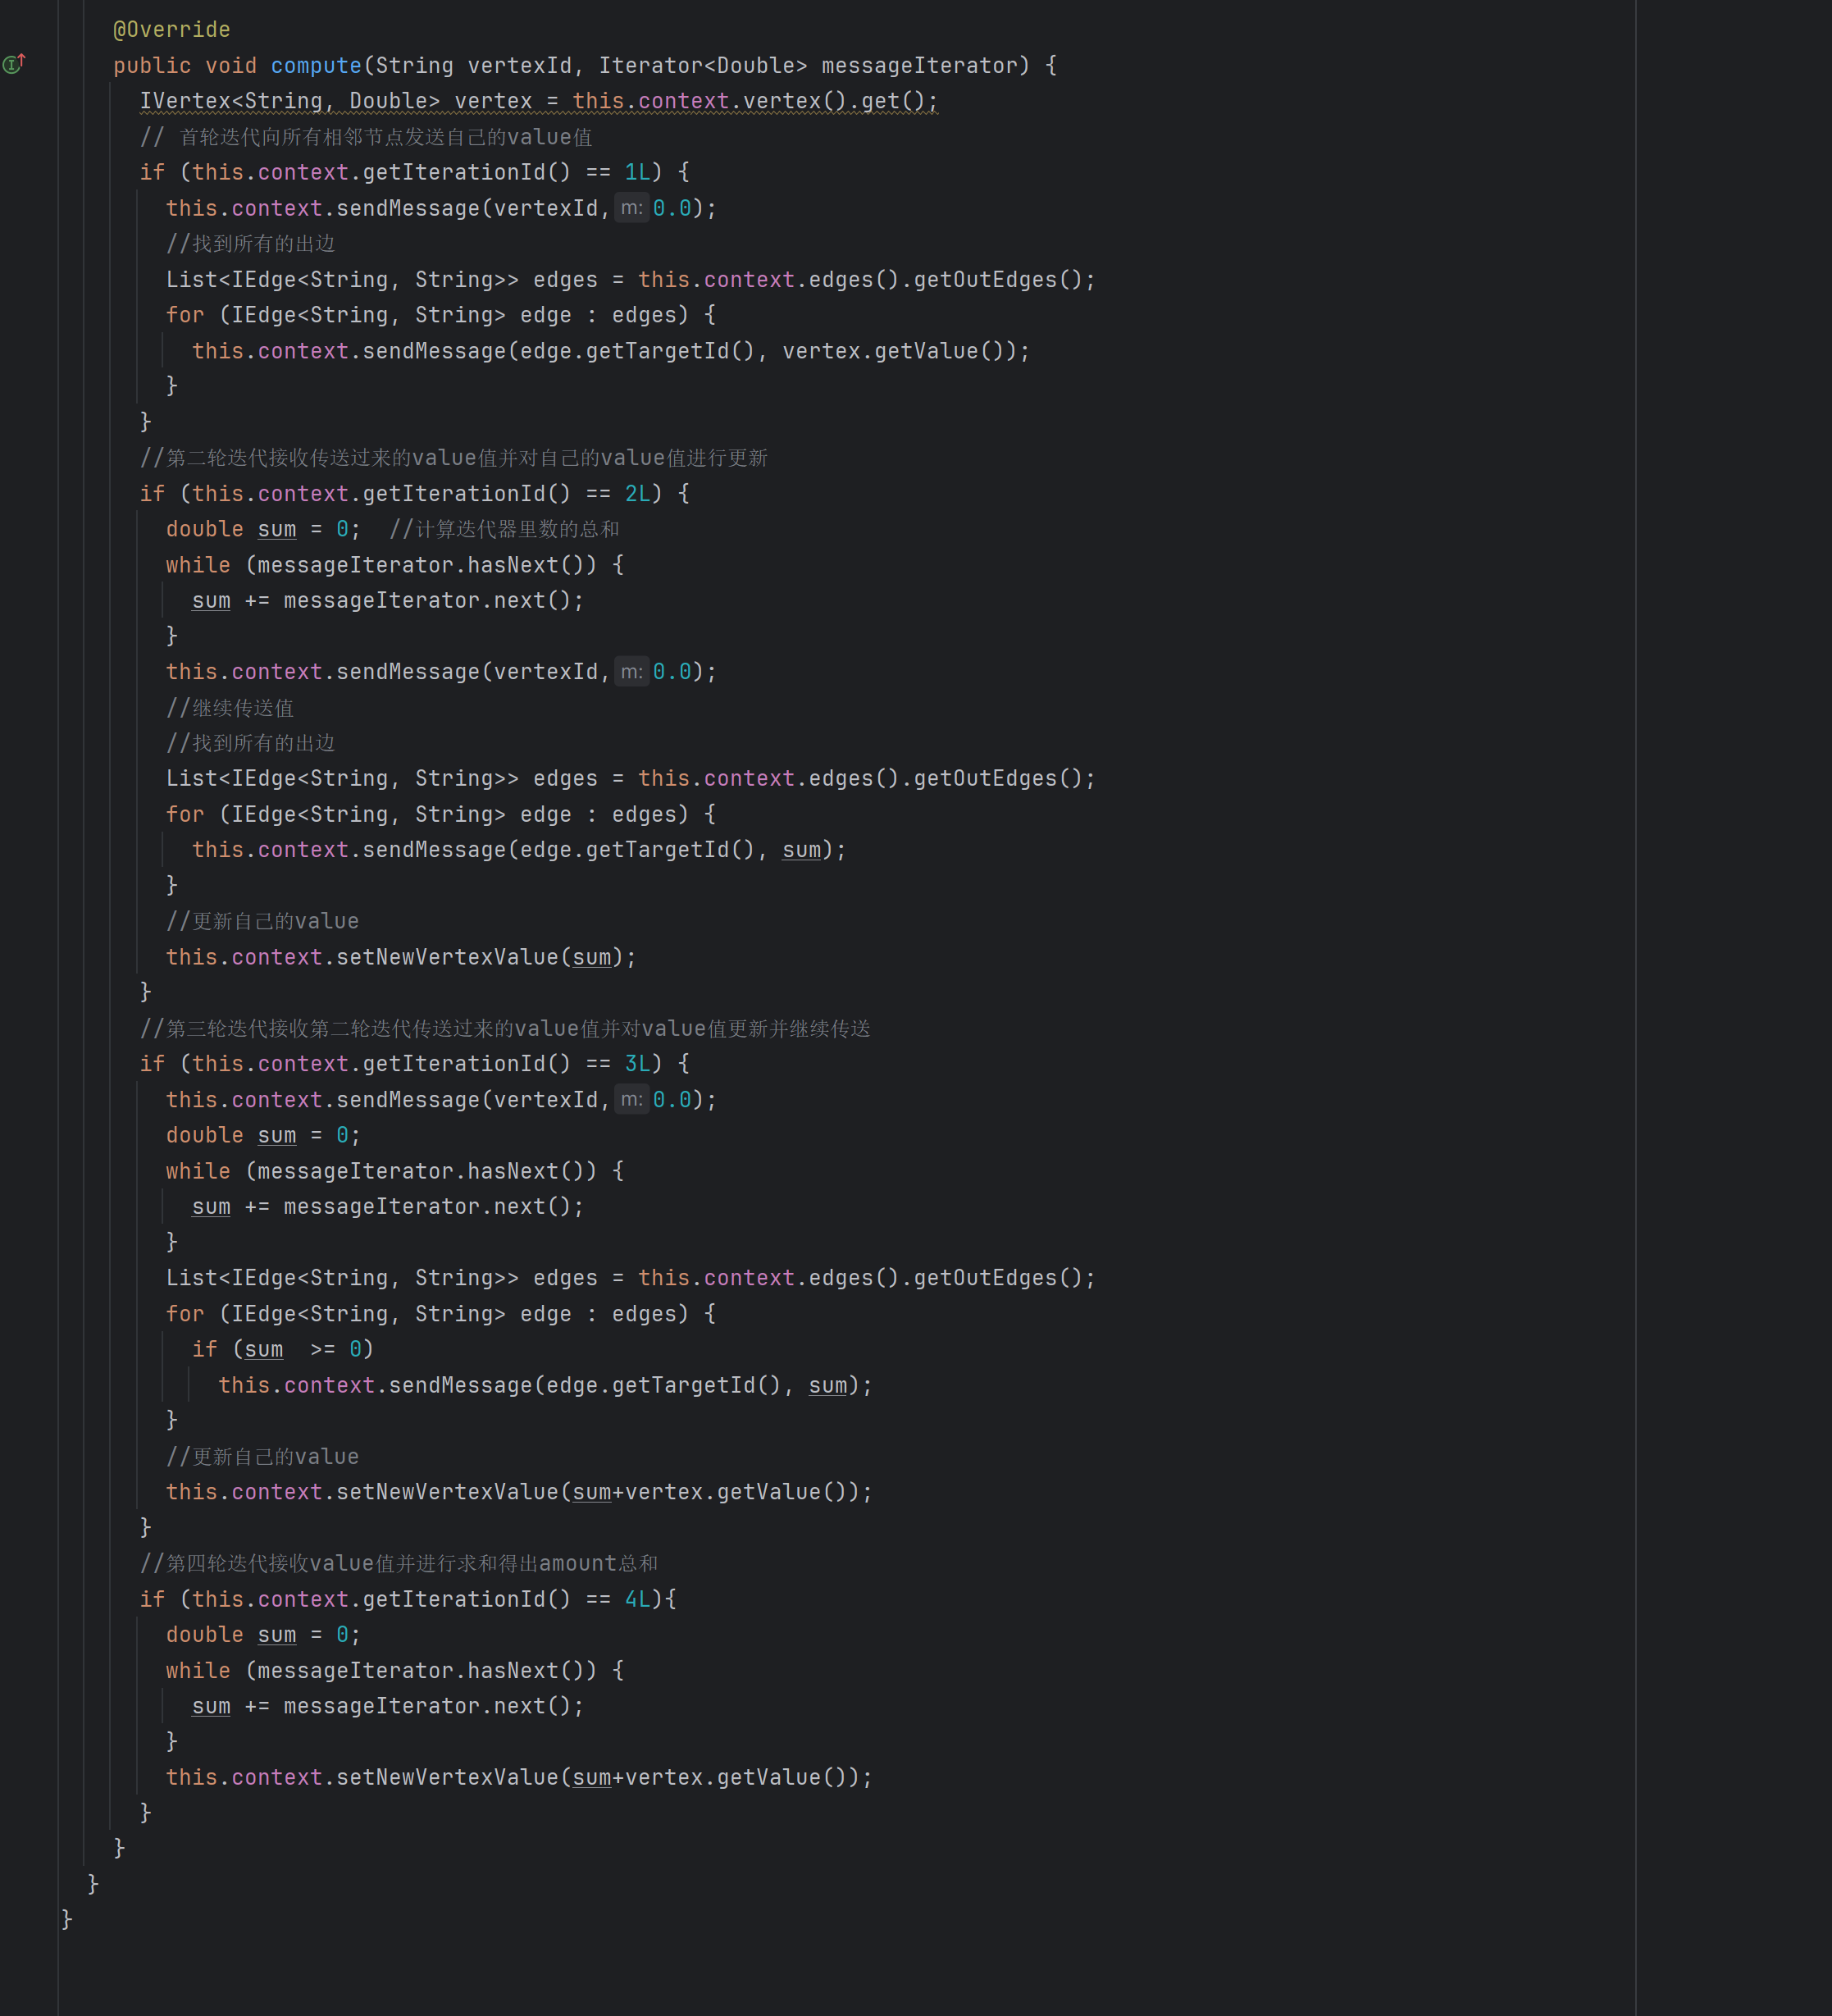
\includegraphics[width=0.85\textwidth,scale=0.7]{./figures/pro3/5.png}
  \end{center}
\end{figure}

最后将结果保存到文件中
\begin{figure}[H]
  \begin{center}
    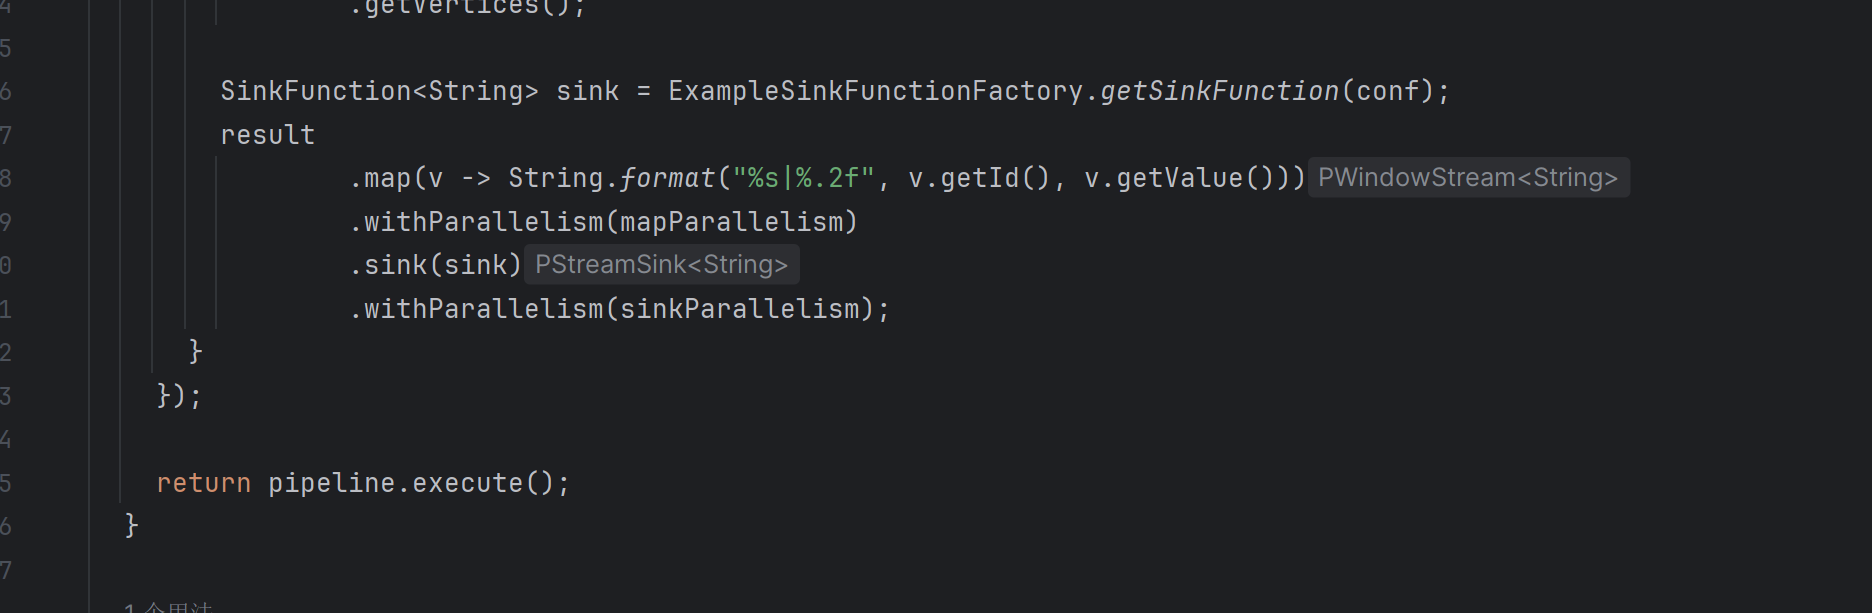
\includegraphics[width=0.85\textwidth,scale=0.7]{./figures/pro3/6.png}
  \end{center}
\end{figure}

但是,提交结果以失败告终了,经过分析,我们发现这个算法不能处理环的问题,因为如
果图中存在环,那么有的点的value值就会就会计算两遍。

\subsubsection{尝试代码优化改进}
上面的算法存在问题,所有我们进行思考后,决定改进第二步操作的compute算法,我们
将点封装成对象,并在迭代中将传递的数据类型改为string类型,可以来判断发送点的具体
信息,用set可以进行点的去重,判断发送源点是否已经给自己发送过数据。每个点首轮
向邻居发送一个消息(点id,1,0.00),当一个点收到消息后若消息的第二个元素
为1或2则直接给消息第一个元素对应的点发送自己的value并将第二个元素加1
传递给邻居;若第二个元素为3,则发送value而不继续传递;最后第二个元素
为4的就是担保链上所有的点发来的消息。
点的类描述如下:
\begin{figure}[H]
  \begin{center}
    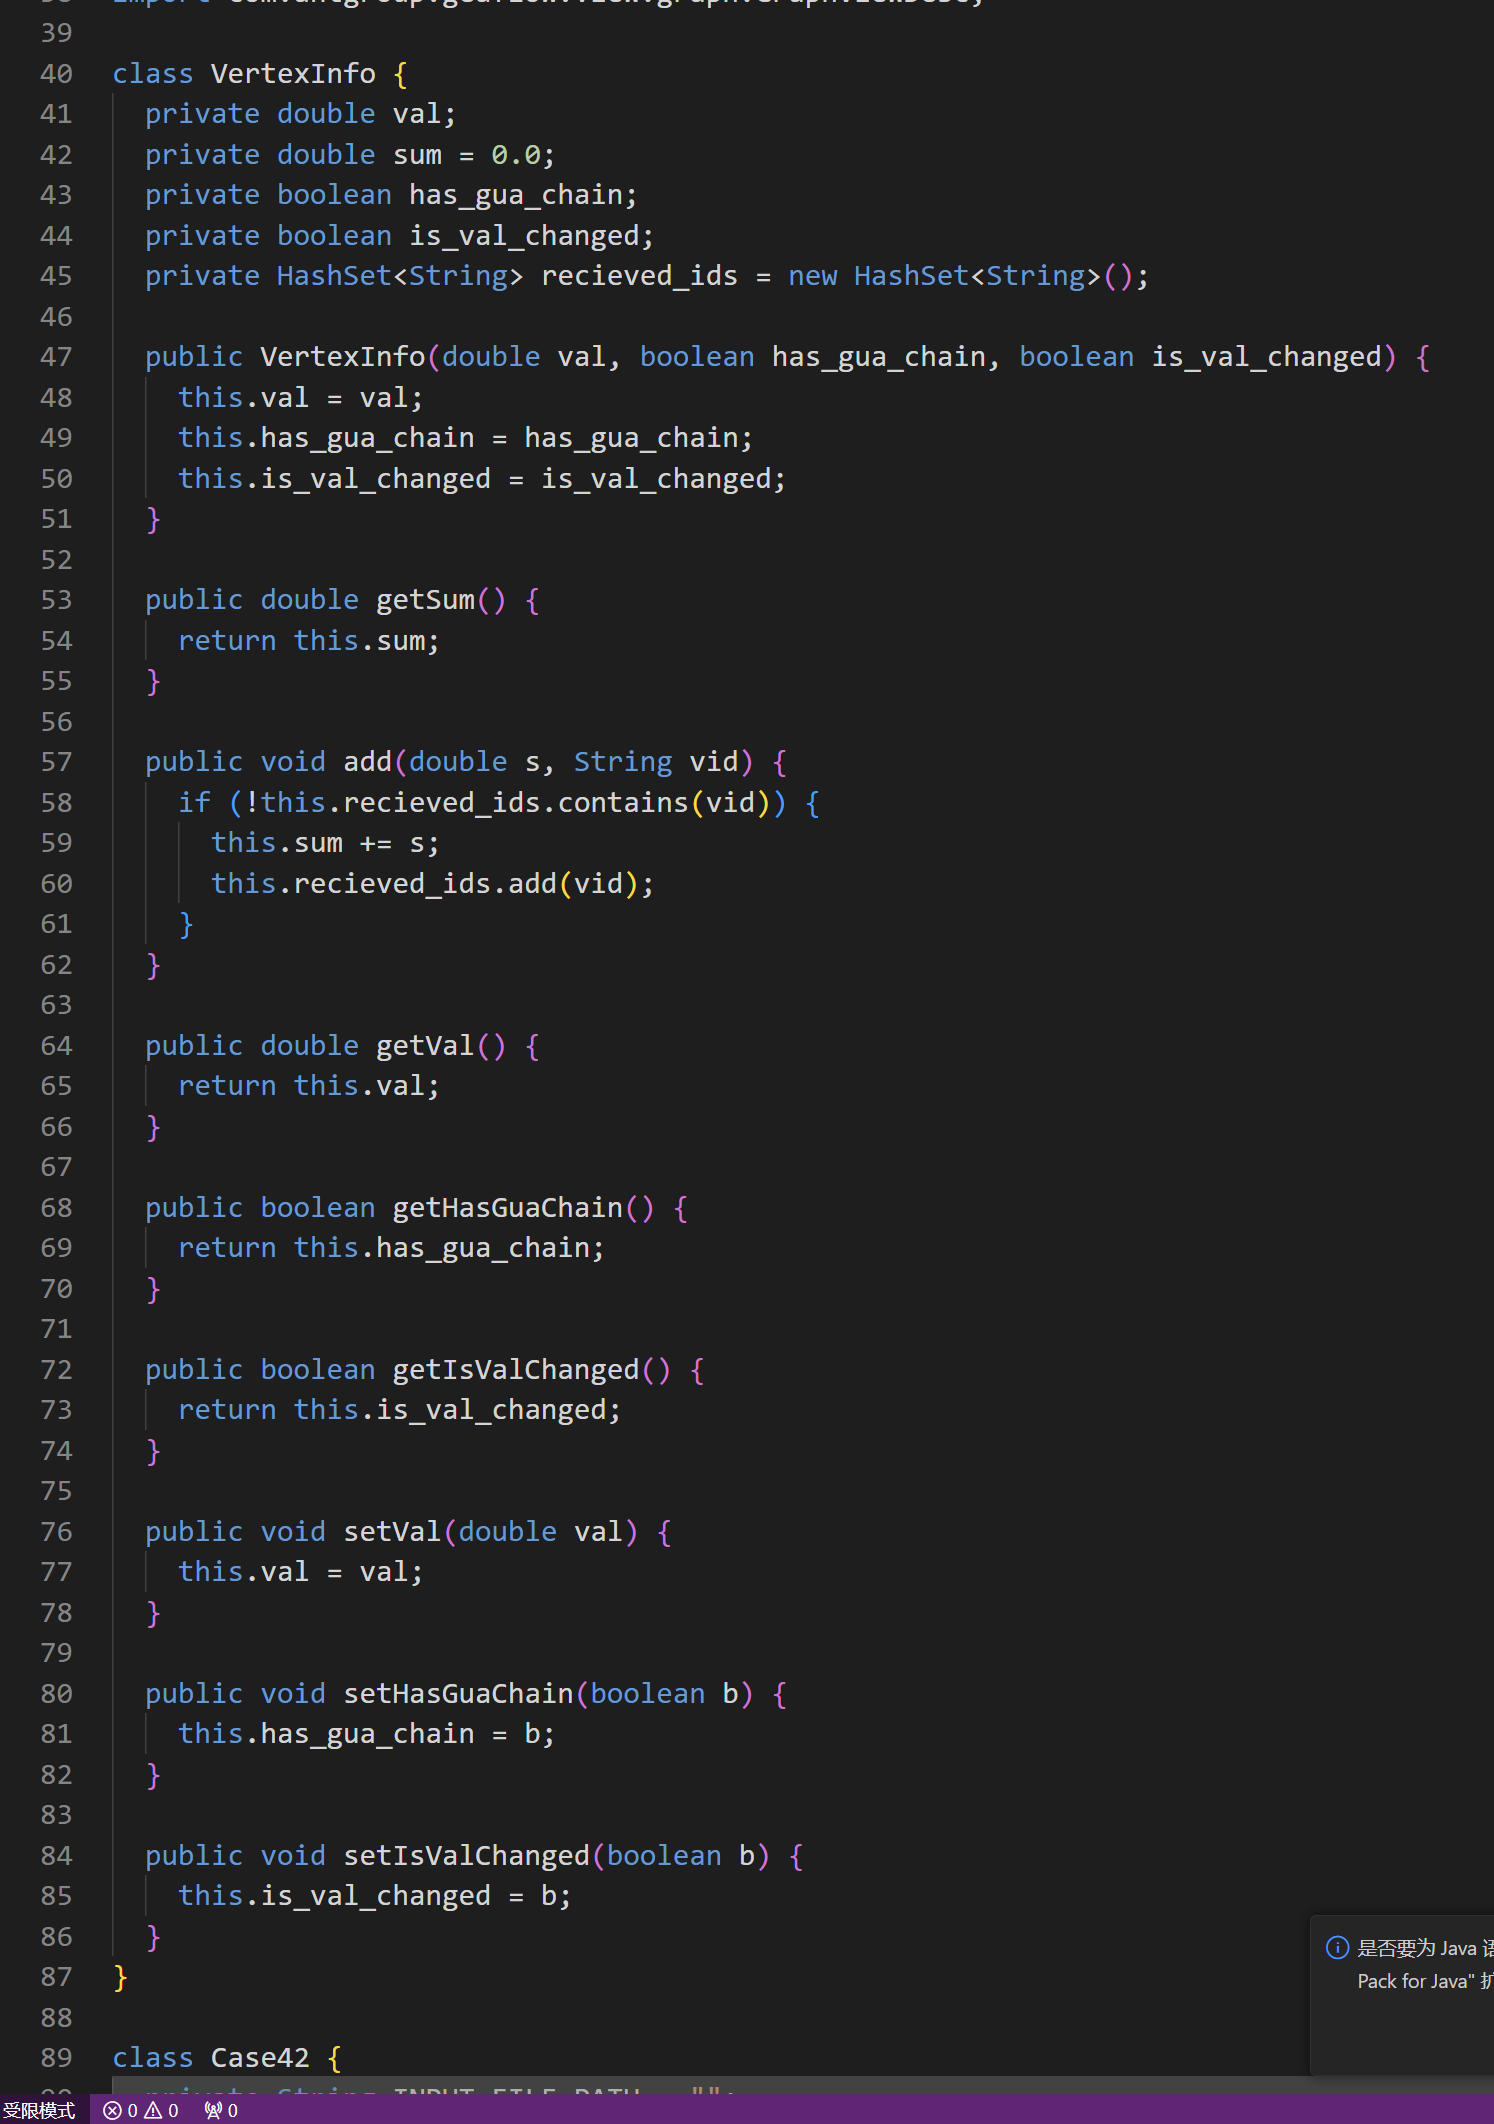
\includegraphics[width=0.85\textwidth,scale=0.7]{./figures/pro3/7.png}
  \end{center}
\end{figure}

更新后的compute如下:
\begin{figure}[H]
  \begin{center}
    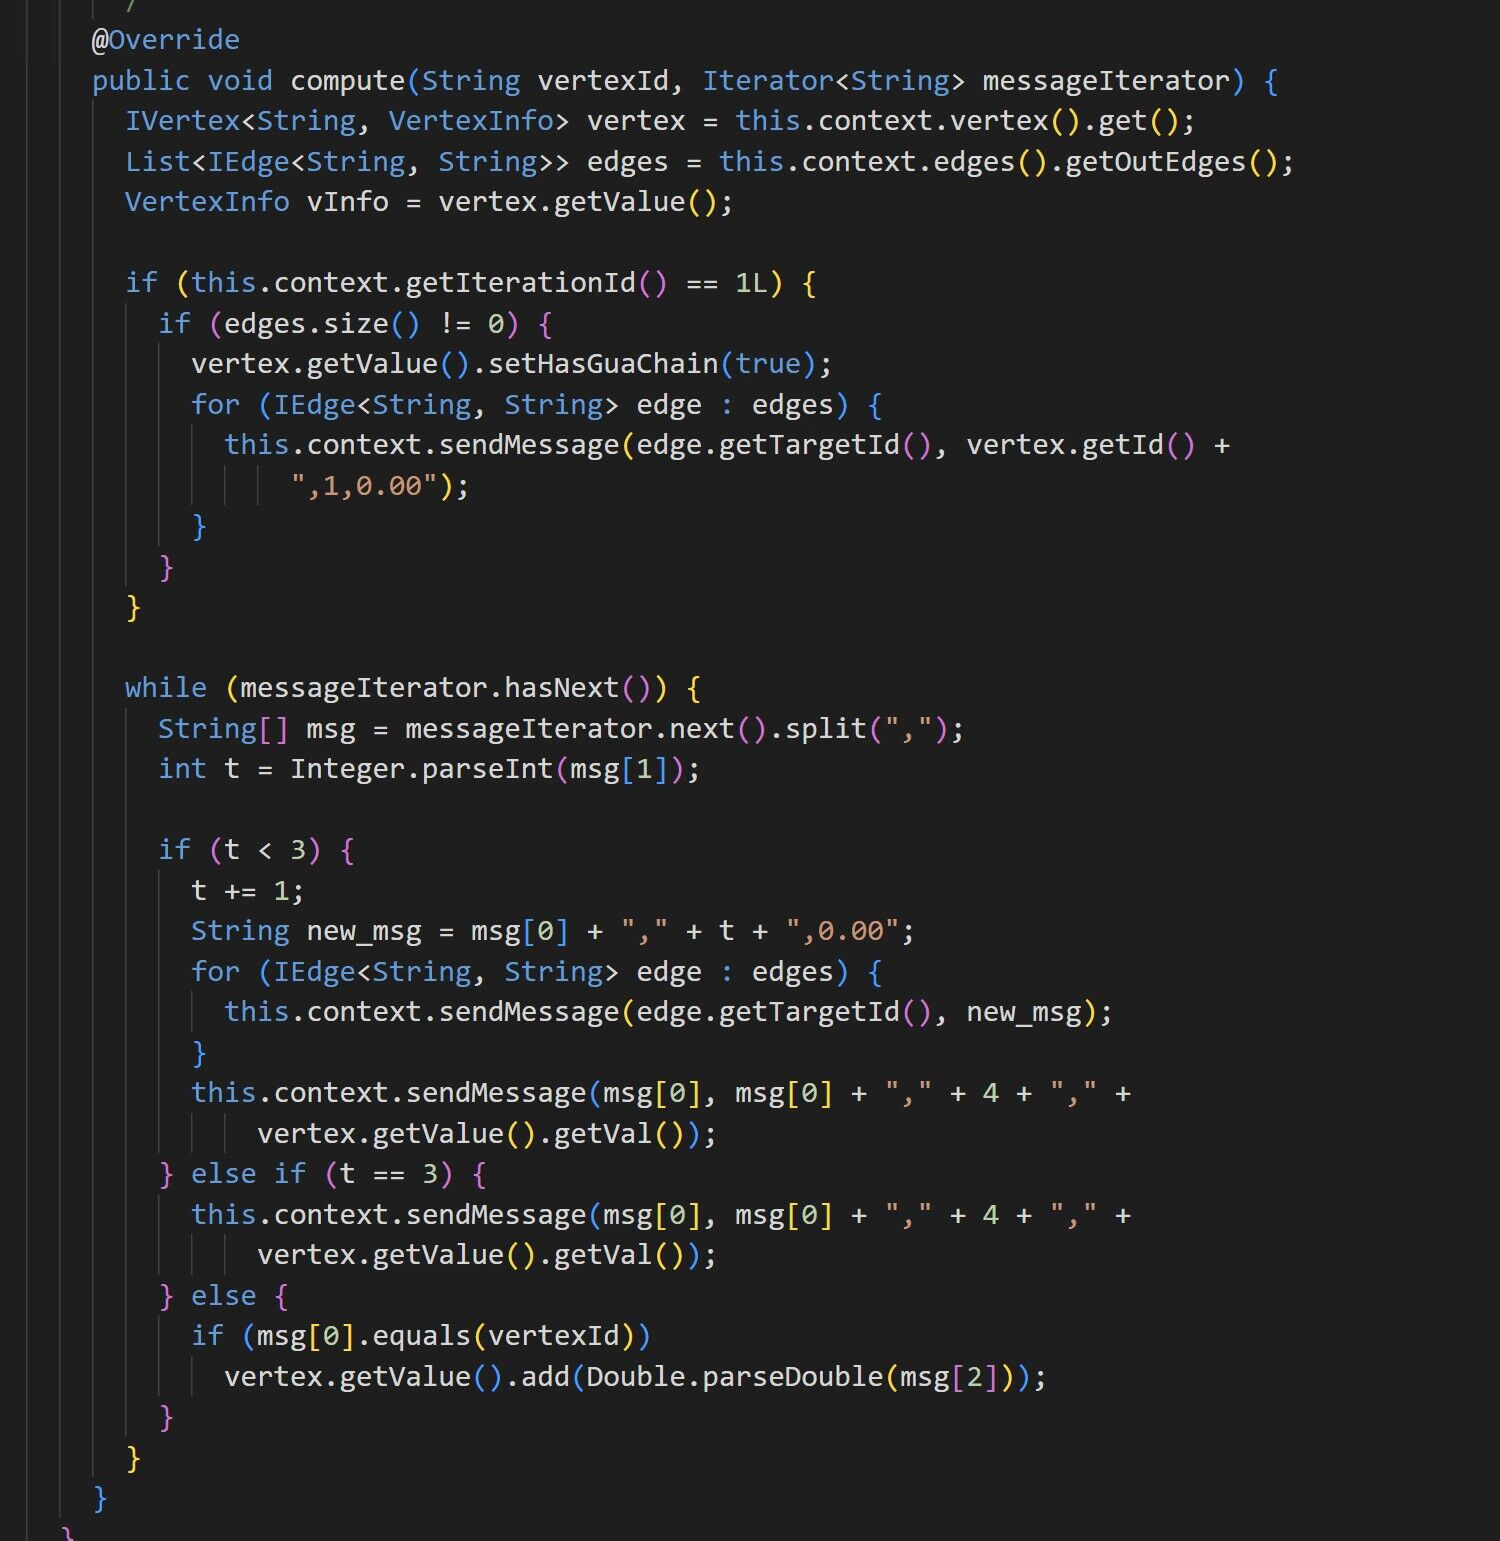
\includegraphics[width=0.85\textwidth,scale=0.7]{./figures/pro3/8.png}
  \end{center}
\end{figure}

我们尝试自己创建文件将自己能想到的所有情况进行测试,结果均正确。但是依然过不了
测试,宣告本题以失败告终。但是在尝试过程中也收获了许多知识点。
